\section{Representation}

In this section, we discuss the representation derived used by \sys to enable
more performant and accurate content-based audio retrieval.
%
~\cref{alg:overall} illustrates the overall flow of the data encoding pipeline.
%
Our goal is to transform the audio waveform into a usable representation for
classification.
%
We next discuss the different stages of the encoding pipeline in detail.

\begin{algorithm}[t!]
    \caption{Construct audio representation for classification.}
	\label{alg:overall}
    \SetKwInOut{Input}{Input}
    \SetKwInOut{Output}{Output}
    \SetKwProg{EncodeAudio}{EncodeAudio}{}{}
    \SetAlgoLined
    
    \EncodeAudio{$(A)$} {
        \Input{Audio recording $A$.}
        \Output{A feature vector $F$ of one or more audio events.}
        $LA \gets LoadAudio(A)$\\
        $TA \gets Tokenize(LA)$\\
        \ForEach{$t_i \in $TA} {
            $F \gets FeatureExtract(t_i)$
        }
        $\Return$ $F$
    }
\end{algorithm}

\subsection{Peripheral Analyzer}
\label{sec:analyzer}

\begin{algorithm}[t!]
    \caption{Tokenize audio recording.}\label{encoder}
    \SetKwInOut{Input}{Input}
    \SetKwInOut{Output}{Output}
    \SetKwProg{Tokenize}{Tokenize}{}{}
    \SetAlgoLined
    
    \Tokenize{$(A)$} {
        \Input{Mono audio recording $A$.}
        \Output{A list of audio frames $L$ in the recording.}
        $A \gets Downsample(A)$\\
        $A \gets Low-Pass(A)$
        $A \gets HalfwaveRectification(A)$\\
        $A \gets Normalize(A)$\\
        $A \gets GetMelCoefficients(A)$\\
        $S \gets SplitOnSilence(A)$\\
        \ForEach{$s_i \in $S} {
            $l \gets A[s_i]$\\
            $L \gets MakeFrames(l)$\\
        }
        $\Return$ $L$
    }
\end{algorithm}

This component is analogous to the cochlea in biological hearing as discussed
in~\autoref{motivation:machine-hearing}.
%
It is responsible for the bulk of the preprocessing on a given audio recording
to construct an usable representation for classification.
%
These preprocessing steps include: 
(1) applying a low-pass filter on the waveform, 
%
(2) downsampling the audio to 16~kHz to only retain the information-dense
frequency range, 
%
(3) decoupling the audio into multiple sources which are then tokenized into a
predefined window of time, 
%
(4) and converting the tokens to a normalized half-wave rectified 
representation to further accelerate query processing.
%
We next describe these steps in detail along with the reasoning behind the 
key design decisions in the peripheral analyzer.

\PP{Downsampling}
%
To improve performance of the encoding algorithm, the peripheral analyzer first 
downsamples the audio signal from its original sample rate.
%
Since the most information dense range of hearing is below 8~kHz\AJ{Cite?},
we only retain those frequencies after downsampling.
%
As per the Nyquist sampling theorem\AJ{Cite?}, the sampling rate must be at
least twice the highest frequency that must be retained:
\begin{equation} \label{eq:nyq}
    f_{sampling} = f_{max} * 2
\end{equation}

In the machine hearing domain, since we only want to retain frequencies below
8~kHz, the optimal sampling rate is 16~kHz. 
%
This does not solve the problem of \textit{aliasing}, 
in which higher frequency components of the signal at lower sampling rates
create aliases of a lower frequency signal.
%
We resolve this aliasing problem by band-limiting the signal to 8~kHz,
effectively removing data at the highest frequency. 
%
Through these steps we are able to reduce the number of samples by upto
64\%\AJ{Min--Max?} while still retaining the critical information.

\PP{Frequency-time series representation}
%
An audio recording can be stored using two representations: (1) amplitude-time
series representation and (2) frequency-time series representation.
%
We choose the latter representation since it better exposes audio structures.
%
We next tailor the frequency-timeseries representation using a \textit{filter
bank}\footnote{A filter bank determines the weights assigned to different
frequencies in the signal.}.
%
We do not use a \textit{standard spectral filter-bank} that gives all
frequencies equal weight in the representation.
%
We instead use the Mel-scale filter bank as it more closely maps the frequency
representation to the perceptual scale of pitches in human hearing\AJ{Cite?}.
%
This filter bank is more discriminative at lower frequencies and 
less discriminative at higher frequencies.
%
We calculate the Mel (\textbf{\textit{m}}) using ~\cref{eq:meleqn}:
\begin{equation} \label{eq:meleqn}
    \textit{m} = 2595 * log_{10}(1+\textit{f}/700)
\end{equation}
%
\AJ{Here, $f$ represents the frequency of the signal.}
%
The corresponding spectrum that we pull the features from gives more weight to
frequencies that are important to human hearing.

\PP{Source Separation Algorithm}
%
An audio recording is made up of a collection of many distinct signals.
%
In order to correctly classify the recording, we must consider this when
creating a representation. 
%
Thus, a \textit{source separation} algorithm is applied to the audio recording
and the separate sources are treated as two distinct signals. 
%
This problem is also referred to as the "cocktail party problem", as in this
situation we have many speakers as well as glasses clinking, people moving, etc.
% 
To solve this problem, we elected to use independent component analysis (ICA).
%
This algorithm separates out components of a mixed signal into its parts.
%
However, one drawback of this technique is that it makes the assumption that 
the sources are statistically independent of each other. 
%
ICA defines independence as the minimization of mutual information given
by~\cref{eq:mutinf} and maximization of non-Gaussianity (to avoid identifying
noise as a component):
\begin{equation} \label{eq:mutinf}
    I(X;Y) = \sum\sum p(x,y)\log(p(x,y)/p(x)p(y))
\end{equation}
%
\AJ{Here, $p(x)$ and $p(y)$ represent the two component signals.}

\PP{Splitting on Silence}
%
To bound the computational load per audio recording, we segment it into
non-silent intervals.
%
We define silence as any interval within the signal below 60~db. 
%
We treat each non-silent interval as an unique audio segment.
%
Otherwise, the classifier may be confused by the hard transitions between
segments.
%
The benefits of removing silence are twofold.
%
First, we improve computational efficiency by not expending compute resources 
on silent intervals.
%
Second, we increase the classifier's accuracy by skipping the silent intervals.

\PP{Half-wave Rectification}
%
To further improve computational efficiency, the audio signal is half-wave
rectified.
%
Half-wave rectification sets negative portions of a signal to zero. 
%
In audio, much of what is expressed in the positive part of the signal is 
simply mirrored on the negative axis\AJ{Cite?}. 
%
Thus, by zeroing out the negative axis of the signal we reduce the amount of
computation needed for each audio recording during feature extraction.

\PP{Windowing}
%
Two key questions related to discrimination of general auditory events are: 
(1) how much of our ability is from discrimination of the spectrum, and 
(2) how much is from temporal evolution of the sound.
%
Prior research has shown that interactions are perceived in the temporal domain
while objects are determined by the frequency domain\AJ{Cite?}. 
%
As we aim to create a classifier with the ability to distinguish between 
general audio recordings, our feature vectors must take time into account. 
%
Thus, we window the audio recording to retain temporal features.

\subsection{Audio Features}

\begin{algorithm}[t]
    \caption{Extract features from an audio segment.}
    \label{alg:encoder}
    \SetKwInOut{Input}{Input}
    \SetKwInOut{Output}{Output}
    \SetKwProg{FeatureExtract}{FeatureExtract}{}{}
    \SetKwProg{EncodeAudio}{EncodeAudio}{}{}
    \SetAlgoLined
        
    \EncodeAudio{$(P)$} {
        \Input{An audio token T.}
        \Output{A vector of extracted features.}
        $T \gets LoadAudioToken(T)$\\
        $TT \gets Tokenize(T)$\\
        \ForEach{token $t_i \in $TT} {
            $F \gets FilterBank(t_i)$ \\
            $F' \gets FeatureExtract(F, t_i)$
        }
    }
\end{algorithm}

\begin{table}[t!]
\centering
%\small
\begin{tabular}{lll}
	\toprule
    Name & Description                       & No. desc. \\
	\midrule
    mvn  & mean, variance, and noise         & 3         \\
    mvnd & mean, variance, noise, derivative & 12        \\
    \bottomrule
\end{tabular}

\caption{
 Descriptors extracted from the audio window by
 aggregating frame features using the above techniques. }
\label{tab:stats}
\end{table}

\begin{figure*}[t]
    \centering
    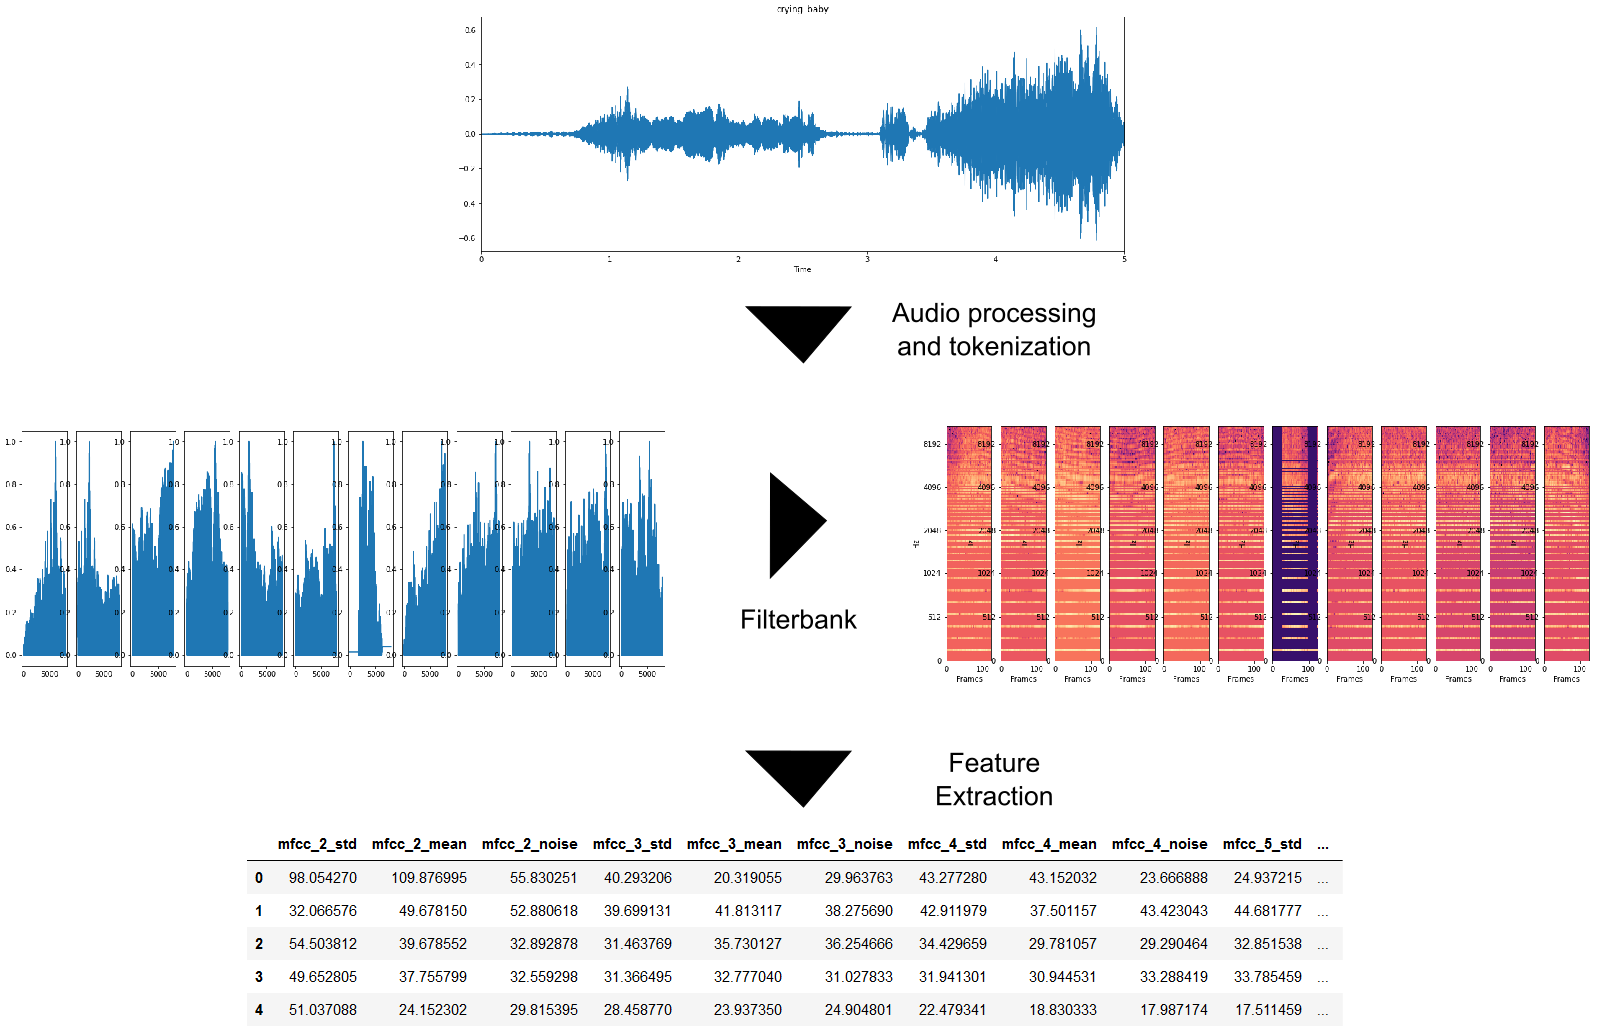
\includegraphics[width=0.7\textwidth]{figures/processing-pipeline.png}
    \caption{File processing pipeline.}
    \label{fig:my-label}
\end{figure*}

We present the set of features that we extract for facilitating audio retrieval
in~\cref{sec:representation::extraction}.
%
We next discuss how we transform these features and select a subset of the
transformed features that best suit the goals of system
in~\cref{sec:representation::transform}.

\subsubsection{Feature Extraction}
\label{sec:representation::extraction}

The feature set consists of both spectral and temporal features. 
%
Most of the chosen features are collected at a per-frame level (\ie, 
a matrix of values over the time window). 
%
All the features are extracted from short-time windows as described earlier.
%
The set of collected features include:

\squishitemize

\item \textit{Mel-frequency cepstral coefficients (MFCC)} capture the timbre
of the audio token. 
%
We use the first 13 coefficients calculated from a 40-channel filter bank.
%
The Mel-scale filter bank closely maps to the perceptual scale of pitches in
human hearing, as discussed in~\cref{sec:analyzer}. 

\item \textit{Spectral centroid} is the balancing point of the spectral power
distribution.

\item \textit{Spectral bandwidth} is the estimated bandwidth of the signal.

\item \textit{Spectral roll-off} captures the skew of the spectral shape. It
computes the frequency below which a certain amount of the spectral energy
resides.

\item \textit{Spectral flatness} The rationale behind this acoustic activity
detector is that the observed signal spectrum evinces more 'structure' when the
signal of interest is present compared to when it is absent.
%
This increase in the structure of the signal may be characterized by a 
reduction in the flatness of the magnitude spectrum of the signal\AJ{Cite?}.
%
Thus, setting an appropriate threshold on the flatness allows for detection of
the presence of the target signal.

\item \textit{Zero-crossing rate (ZCR)} is a measure of the number of zero
voltage crossing within an audio frame (obtained before half-wave
rectification).

\item \textit{Short-time average energy} is the sum of squared amplitudes 
within a frame representing the energy of a frame.

\item \textit{Root Mean Squared Energy} is the square root of the arithmetic
mean of the squares of the values, or the square of the function that defines the
continuous waveform.

\squishend

\PP{Matrix to Vector Transformation}
We apply statistical techniques to reduce this matrix to a vector. 
%
To reduce the representation to a vector while still retaining the data, we
collect a combination of statistics. 
%
We evaluate several combinations to determine the one that provides the most
information-dense feature vector. 
%
~\cref{tab:stats} summarizes the tested combinations of feature statistics 
and the number of derived descriptors.
%
\AJ{As many of these features are collected at a frame level statistics, found
in~\cref{tab:stats}, are computed over the entire window. --?}

\subsubsection{Feature Transformation}
\label{sec:representation::transform}

With all the collected and statistically-derived features, the vector contains
around 129 values.
%
Such a long vector presents an issue in training and evaluating classifiers
(\ie, the curse of dimensionality)\AJ{Cite?}.
%
We shrink the vector by applying feature selection and reduction techniques as 
a final preprocessing step.
%
Through experimentation, we found that the chi-square test and principal
component analysis to be the most effective techniques for feature selection and
reduction, respectively.

\PP{Feature Selection} 
%
We compute chi-squared stats between each non-negative feature and class.
% 
The chi-square test weeds out the features that are the most likely to be
independent of class by measuring the dependence between stochastic variables.
%
Thus, it selects the subset of features that are relevant for classification.

\PP{Feature Reduction}
%
We reduce the feature set using \textit{principal component analysis} (PCA).
%
PCA uses orthogonal transformations to convert a feature set of 
possibly correlated variables into a set of linearly uncorrelated variables
known as principal components. 
%
This technique allows us to provide a number of desired principal components,
thereby reducing the number of features in a controlled manner. 
%
However, the optimal number of principal components depends on the dataset 
and must be carefully chosen as the features may already be of sufficient
variance and dropping any will reduce the efficacy of the model. 
%
% This is an iterative technique with the first component being computed thus:
% \begin{equation}
%     \textbf{w}_{(1)} = \argmax_{||\textbf{w}||=1}{\sum_{i}(\textbf{x}_{(i)} \cdot \textbf{w})^2}
% \end{equation}
% %
% Here, \textbf{x} is a row vector of input data \textbf{X} and \textbf{w} is 
% the coefficient vector, constrained to be the unit vector. 
% %
% The subsequent components are computed by subtracting the first \textit{k} - 1
% principal components from \textbf{X} thus:
% \begin{equation}
%     \hat{\textbf{X}}_k = \textbf{X} - \sum_{s=1}^{k-1}{\textbf{X}\textbf{w}_{(s)}\textbf{w}_{(s)}^\textbf{T}}
% \end{equation}
% %
% and afterward finding a weight vector that extracts the maximum variance from
% the new data matrix:
% \begin{equation}
%     \textbf{w}_{(\textit{k})} = \argmax_{||\textbf{w}||=1}(||\hat{\textbf{X}}_{\textit{k}}\textbf{w}||^2)
% \end{equation}
% %
% It turns out in that the weight vectors computed using this iterative technique
% are eigenvectors of $ \textbf{X}^\textbf{T}\textbf{X} $.
%
We demonstrate that these feature transformation techniques effectively
shrink the feature vector in~\cref{sec:evaluation-encoding}.

\begin{figure}[t]
    \centering
    \includegraphics[width=0.45\textwidth]{example-image-a}
    \caption{Plot of feature reduced samples from music, animal, speech, and environmental sounds}
    \label{fig:top-dist}
\end{figure}
